\documentclass[11pt,a4paper]{article}
\usepackage{fontspec}
\setmainfont{Source Serif 4}[Path=/home/claude/ref/fonts/, UprightFont=SourceSerif4-Regular.ttf, BoldFont=SourceSerif4-Semibold.ttf, ItalicFont=SourceSerif4-It.ttf]
\setmonofont{IBM Plex Mono}[Path=/home/claude/ref/fonts/, UprightFont=IBMPlexMono-Regular.ttf, BoldFont=IBMPlexMono-Medium.ttf, Scale=0.88]
\usepackage[a4paper,margin=2.4cm]{geometry}
\usepackage{amsmath,amssymb}
\usepackage{graphicx,booktabs,float,caption,array,xcolor,longtable}
\usepackage{xurl}
\usepackage[hidelinks]{hyperref}
\usepackage[round]{natbib}
\usepackage{setspace}
\setstretch{1.08}
\renewcommand{\topfraction}{0.9}
\renewcommand{\bottomfraction}{0.8}
\renewcommand{\textfraction}{0.1}
\renewcommand{\floatpagefraction}{0.75}
\setlength{\parindent}{0pt}
\setlength{\parskip}{0.55em}
\captionsetup{font=small,labelfont=bf}
\setlength{\bibsep}{3pt}
\urlstyle{same}
\hypersetup{pdftitle={Do the Clocks Kill?},pdfauthor={Dr Tristan Hotham}}

\begin{document}
\begin{center}
{\Large\bfseries Do the Clocks Kill? Reported Road Collisions Either Side of the Clock Changes in Great Britain, 1979 to 2025\par}
\vspace{1.2em}
{\large Dr Tristan Hotham\par}
\vspace{0.3em}
{\small Independent researcher\\
ORCID: 0000-0003-4931-9349\\
DOI: https://doi.org/10.5281/zenodo.24112857\par}
\vspace{0.8em}
2026
\end{center}

\begin{quote}
\small
\begin{center}\textbf{Abstract}\end{center}
Twice a year Britain moves its clocks, and the press asks whether crashes follow. Two mechanisms are usually proposed: a lost hour of sleep after the spring change, and an hour of evening darkness moved into the commute after the autumn change. I test both with every personal-injury road collision reported to the police in Great Britain from 1979 to 2025 (9,116,617 collisions), with an analysis plan written in advance. For 91 clock changes I compare the week after each change with the same weekdays in the three weeks either side, and, within each day, the share of collisions falling in the evening and morning hours whose light the change moves. In the week after the clocks go forward, collisions changed by 0.8\% (95\% CI -1.5 to 3.1); in the week after they go back, by -0.1\% (-2.3 to 2.1). Fatal collisions after the autumn change were 4.2\% higher (-0.3 to 8.9), an estimate matched by 2 of 29 placebo weeks. The autumn change raised the share of evening-peak collisions recorded in darkness from 68\% to 88\%, yet collisions in those hours rose only 3.9\% relative to midday, a shift that ordinary weeks produce about one time in 4; the spring evening moved the wrong way for a darkness effect, and an exploratory step at both changes is not explained by light. The clock changes are not followed by a detectable rise in reported injury collisions in Britain; any fatal effect is small and uncertain.

\textbf{Keywords:} daylight saving time; British Summer Time; road traffic collisions; ambient light; STATS19; natural experiment
\end{quote}

\section{Introduction}\label{sec:intro}
On the last Sunday of March the clocks in the United Kingdom go forward by one hour, and on the last Sunday of October they go back. Each change is followed by a familiar news story: drivers are tired, evenings are suddenly dark, and road safety charities warn of more crashes. The claim has two separate parts. The first is about sleep. Moving the clocks forward costs most people an hour in bed on the Saturday night, and tired drivers make mistakes \citep{harrison2013,kantermann2007}. The second is about light. Because people keep to clock time, the change moves an hour of daylight between the morning and the evening. In spring the evening commute moves into daylight and the morning commute towards darkness; in autumn the reverse. Darkness is a well-established risk factor on the road, especially for people on foot \citep{plainis2006,sullivan2007,uttley2017aap}, so the light mechanism predicts more crashes in the newly dark hours and fewer in the newly light ones.

These two mechanisms have very different policy implications. A sleep effect is a cost of changing the clocks at all and would argue for abolishing the change in either direction. A light effect is a cost or a benefit of where the hour of daylight sits, and has been used for decades to argue that Britain should keep lighter evenings in winter, as it did in the British Standard Time experiment of 1968 to 1971 \citep{homeoffice1970,broughton1999}. The international evidence is mixed. A systematic review of 24 studies found the short-term effects of the transitions on collisions to be inconsistent \citep{carey2017}. Large studies of United States fatal crashes have found increases of around six per cent in the week after the spring change \citep{smith2016,fritz2020}, but a recent study using states that do not change their clocks as controls found no overall change \citep{lei2026}.

This paper asks the question for Great Britain with the longest and most complete series available: every personal-injury road collision reported to the police from 1979 to 2025, 9,116,617 collisions in all. The design is simple and was written down, with its hypotheses, hour groups, comparison windows, exclusions and robustness checks, before any counts around a clock change were computed (Section~\ref{sec:design}). For each of the 91 clock changes in the main sample I compare the week after the change with the same weekdays in the three weeks before and the three weeks after. A second set of models looks inside each day: with a fixed effect for every calendar day, they compare only the share of each day's collisions falling in the evening (17:00 to 18:59) and the morning (06:00 to 08:59) with the share in the middle of the day, which removes weather, holidays and other whole-day shocks. Finally, the same models are run on 29 groups of ordinary Sundays, as if the clocks had changed on them, to see how large an apparent effect normal weeks produce.

The answer is mostly no. In the week after the clocks go forward, reported injury collisions changed by 0.8\% (95\% CI -1.5 to 3.1); in the week after they go back, by -0.1\%. Neither is distinguishable from zero, and both look like the changes seen after ordinary Sundays. The one estimate that leans towards harm is for fatal collisions after the autumn change (4.2\%, CI -0.3 to 8.9), which is as large as all but 2 of the 29 placebo estimates. The light mechanism is clearly visible in what police recorded: after the autumn change the share of evening-peak collisions in darkness jumps from 68\% to 88\%. But the number of collisions in those hours rises only 3.9\% relative to the middle of the day, and in spring, when the evening peak becomes lighter, its share of collisions rose rather than fell.

The paper contributes in three ways. It is, to my knowledge, the first analysis of the British clock changes that uses the whole STATS19 series from 1979 to 2025 with a single pre-specified design, giving 47 years of changes and 45 to 46 changes per season in the main sample. It separates whole-day effects from the reallocation of collisions between hours with day fixed effects, and it reports both against a placebo distribution built from the same data, which shows how easily ordinary calendar weeks generate apparent effects of a few per cent. And it reports a careful null: for a policy debate in which large numbers are often quoted, it shows how small the short-run effects of the changes on reported collisions in Britain are.

Section~\ref{sec:lit} reviews the literature. Section~\ref{sec:data} describes the data and the clock-change dates, Section~\ref{sec:design} the pre-specified design, Section~\ref{sec:results} the results and Section~\ref{sec:robust} the placebo and robustness checks. Section~\ref{sec:disc} discusses what the results mean and what they cannot show, and Section~\ref{sec:conc} concludes.

\section{Background and literature}\label{sec:lit}
\subsection{The British clock}
Great Britain has observed summer time since 1916. Under the Summer Time Act 1972 \citep{summertimeact1972} and the European harmonisation that followed (Directive 2000/84/EC, \citealp{eu2001}, implemented in the Summer Time Order 2002), clocks go forward at 01:00 GMT on the last Sunday of March and back at 01:00 GMT on the last Sunday of October. Before 1996 the autumn change came earlier, on the day after the fourth Saturday of October, and in 1979 and 1980 the spring change was in mid March. From 27 October 1968 to 31 October 1971 the country tried British Standard Time, keeping GMT plus one hour all year. The official review of the experiment reported an overall improvement in road casualties during the relevant times of day, but, as the Home Secretary's answer to Parliament summarised it, ``the crude figures of savings of casualties need to be treated with reserve'' \citep{homeoffice1970,hansard1970}. Other road safety measures arrived shortly before the experiment, among them the roadside breath test introduced by the Road Safety Act 1967, which complicates any before-and-after comparison. That experiment ended before the STATS19 series used here begins and is not analysed in this paper.

\subsection{Light and road risk}
The risk of a collision is higher in darkness than in daylight for the same road and traffic, and the excess is largest for pedestrians \citep{plainis2006,sullivan2007}. Because travel and darkness are both strongly patterned by time of day and season, the effect of light is hard to separate from that of traffic, fatigue and alcohol. The clock changes offer a way in: for an hour or so around each commute, the change moves the light while, if people keep to clock time, the traffic stays the same. \citet{sullivan2002} used the United States transitions in this way to infer the role of ambient light in fatal crashes, and \citet{johansson2009} formalised the comparison as a case hour, whose light changes across the transition, set against control hours whose light does not. \citet{uttley2017aap} applied the method to British pedestrian collisions on crossings, using STATS19 records from 2005 to 2015. For Britain as a whole, \citet{broughton1999} modelled casualties by week and hour against solar altitude for 1969 to 1973 and 1985 to 1994 and used the estimates to predict the effect of alternative clock schedules, building on the TRL assessment of single/double summer time \citep{broughton1998}. \citet{bunnings2021} estimated that darkness imposes annual costs of £790 million on British roads and that year-round summer time could save about a tenth of them.

The assumption that people keep to clock time is not exact. \citet{uttley2017jep} used the clock change to show that daylight raises the number of people walking and cycling, so exposure itself moves with the light. A rise in collisions in a newly lit hour can therefore reflect more people out, not more risk per person.

\subsection{Sleep and the spring transition}
The spring change shortens the night for most people, and the circadian system takes days to adjust \citep{kantermann2007,harrison2013}. Short-term health effects have been reported for heart attacks \citep{janszky2008} and for workplace injuries \citep{barnes2009}. For roads, early studies of United States and Canadian data reported more crashes on the Monday after the spring change \citep{coren1996,hicks1983}, while others found no effect \citep{lambe2000,lahti2010}. \citet{varughese2001} reported a rise in fatal crashes on the Monday after the spring change in United States data. \citet{smith2016} used the discrete transitions and the 2007 change in the United States schedule to conclude that the spring transition ``caused over 30 deaths'' a year from 2002 to 2011, and that ``shifting ambient light only reallocates fatalities within a day'' while sleep loss increases risk. \citet{fritz2020} found a six per cent rise in fatal crashes in the week after the spring change in 732,835 United States fatal crashes from 1996 to 2017, larger at the western edges of time zones. \citet{robb2018} found more road injury claims in the days after the spring change in New Zealand.

\subsection{Recent designs and the British evidence}
Two recent papers sharpen the design question. \citet{lei2026} used Arizona and Hawaii, which do not change their clocks, as controls, and found no change in total fatal crashes after the spring change (+0.2\%) but a rise in morning fatal crashes; they argue that uncontrolled before-and-after comparisons can be confounded by the season. \citet{woods2025} compared the five weeks before and after each change in United States fatal crashes from 2010 to 2019 and found that occupant and pedestrian crashes moved in opposite directions, the pedestrian changes following the light. \citet{laliotis2023} found in Greek data from 2006 to 2016 that entering summer time was followed by fewer serious accidents, concentrated in the evening, and leaving it by more minor accidents, again mainly in the evening, and concluded that road safety alone is not a strong reason to adopt or abolish summer time.

British evidence on the short-run effects of the transitions is thin. \citet{whittaker1996} studied casualties in Cheshire, and \citet{adams2005} examined serious and fatal injuries to children in north-east England. The systematic review by \citet{carey2017} concluded that the evidence ``cannot support or refute the assertion'' that a permanent shift of light from morning to evening would benefit road safety. Further American studies of the transitions and of longer-run effects \citep{meyerhoff1978,ferguson1995,coate2004,sood2007,stevens2006,huang2010} are covered by that review. This paper adds a long British series, a design that separates whole-day from within-day effects, and an explicit placebo distribution.

\section{Data}\label{sec:data}
\subsection{Collisions}
The data are the Department for Transport's road safety data, the STATS19 records of every personal-injury road collision reported to the police in Great Britain \citep{dft2026}. The published collision file covers 1979 to 2025. I use 9,116,617 collisions with 12,102,123 casualties, of which 146,175 were fatal collisions (at least one person died within 30 days). The file was reduced to counts by calendar day, clock hour (the police record local clock time), severity and light condition (daylight, darkness of any kind, or unknown); every collision has a time. Annual counts fell from 254,967 collisions and 5,824 fatal collisions in 1979 to 101,525 and 1,453 in 2025. Damage-only collisions and injury collisions not reported to the police are not included, so the outcome is reported injury collisions, not all crashes.

Severity is not recorded consistently over the whole period. Since 2012 police forces have moved to injury-based reporting systems such as CRASH, which classify severity from the recorded injury; the Department for Transport estimates that the move raised the number of casualties classed as serious by 5 to 15\% across Great Britain \citep{dftseverity2026}. Because this paper compares weeks a few days apart within the same year, the change does not bias the comparisons, but I use only all-injury and fatal collisions, both defined consistently throughout.

For the local analysis, collisions carry the code of the local authority district in which they occurred. Codes are missing before 1994 and partly to 1996, and some districts abolished in 2009 appear only to 2008. From 2009 every code can be mapped to a 2023 district using the successor table of \citet{mysociety2026}, plus three manual mappings (Heathrow to Hillingdon, and the 2025 codes for Barnsley and Sheffield to their previous codes). The local analysis therefore covers 2009 to 2025.

\subsection{The clock changes}
The dates of the changes are taken from the IANA time zone database \citep{iana2026} for Europe/London rather than typed by hand, and checked against known anchors (18 March and 28 October 1979; 22 October 1995; 27 October 1996). Each year has one spring change (clocks forward, the Sunday on which the offset from UTC goes from zero to one hour) and one autumn change, giving 94 changes from 1979 to 2025. Three are excluded in advance because a pandemic lockdown rule began or ended inside their window: spring 2020 (the first lockdown began on 23 March 2020), autumn 2020 (a second English lockdown began on 5 November 2020) and spring 2021 (the stay-at-home rule ended in England on 29 March 2021, the day after the change). The main sample has 45 spring and 46 autumn changes. Table~\ref{tab:data} summarises the data flow.

\begin{table}[tbp]\centering\small\caption{Data and sample.}\label{tab:data}\begin{tabular}{lr}\toprule Item & Number\\\midrule
Reported injury collisions, 1979 to 2025 & 9,116,617\\
\quad fatal collisions & 146,175\\
\quad casualties & 12,102,123\\
Clock changes, 1979 to 2025 & 94\\
\quad excluded in advance (pandemic rules) & 3\\
\quad main sample: spring / autumn & 45 / 46\\
Collisions in the 49-day windows (main sample) & 2,441,460\\
\quad of which fatal & 38,849\\
Collisions in the change weeks (main sample) & 348,932\\
\quad of which fatal & 5,660\\
Placebo Sundays / ISO weeks analysed & 1,290 / 29\\
Districts in the local analysis (2009 to 2025) & 350\\
\bottomrule\end{tabular}\end{table}

\section{Research design}\label{sec:design}
The analysis plan was written in the study notes before any count around a clock change was computed. Deviations are listed in Section~\ref{sec:dev}.

\subsection{Windows}
Day 0 is the Sunday of the change. The treatment week is days 0 to 6. The comparison weeks are the same weekdays one to three weeks before (days $-21$ to $-1$) and one to three weeks after (days 7 to 27). Placing the comparison weeks symmetrically around the change cancels a linear seasonal trend in traffic and daylight, which matters because traffic and the length of the day change steadily through March and October. Day-of-week patterns are absorbed by fixed effects for each change and weekday.

\subsection{H1: the whole week}
For change $e$ and day $d$, the count of collisions $y_{ed}$ is modelled by Poisson pseudo-maximum likelihood \citep{santos2006,correia2020}:
\begin{equation}
E[y_{ed}] = \exp(\beta\,\text{Treat}_{ed} + \gamma\,\text{Holiday}_{ed} + \alpha_{e,\text{dow}(d)}),
\end{equation}
where Treat marks days 0 to 6, Holiday marks bank holidays in England and Wales (Good Friday, Easter Monday and the May and August bank holidays; every spring window contains Easter), and $\alpha$ are change-by-weekday fixed effects. The rate ratio $\exp(\beta)$ compares the change week with the comparison weeks. Standard errors are clustered by year, so that the spring and autumn changes of the same year share a cluster \citep{cameron2015,abadie2023}. Four estimates are planned: spring and autumn, all-injury and fatal. Two secondary estimates test the sleep hypothesis more narrowly: the Monday after the change (day 1 against the comparison Mondays) and the working week (days 1 to 5).

\subsection{H2: light moving between hours}
Darkness should move collisions between hours within a day. The second model counts collisions $y_{edg}$ in four groups of clock hours $g$: evening (17:00 to 18:59), morning (06:00 to 08:59), reference (10:00 to 15:59, light in every week of every window) and other hours. With a fixed effect for every day,
\begin{equation}
E[y_{edg}] = \exp\Big(\sum_{g\neq\text{ref}} \beta_g\,\text{Treat}_{ed}\,\mathbb{1}[g] + \delta_{ed} + \alpha_{eg}\Big),
\end{equation}
the coefficients $\beta_g$ measure the change in a group's collisions relative to the reference hours. The day effects $\delta_{ed}$ absorb anything that shifts a whole day, such as weather, a holiday or a strike, and $\alpha_{eg}$ allow each change its own hour profile. The plan predicts an autumn evening ratio above one and a spring evening ratio below one, with the morning the other way round. A manipulation check reports the share of collisions in each group that police recorded as in darkness, in the comparison and treatment weeks. The full hour-by-hour version, with each hour compared with the reference hours, is used for Figure~\ref{fig:hours}.

\subsection{H3 and H4: darkness risk and the net effect}
Combining the two seasons gives a darkness contrast for the evening hours: half the difference between the autumn coefficient (light to dark) and the spring coefficient (dark to light), estimated in a stacked model so that the covariance between seasons is accounted for. This follows the case-hour logic of \citet{johansson2009} and \citet{sullivan2002}. The net effect (H4) multiplies each group's ratio by its comparison-week count to give the expected number of extra or fewer collisions per change week; it is arithmetic, not a test.

\subsection{Event study and placebo}
For the event-study figure, each day's count from day $-21$ to day 27 is divided by the mean of the same weekday in the comparison weeks (excluding the day itself), pooled over changes, with 95\% intervals from 2,000 bootstrap draws of years. For the placebo, every Sunday in 1979 to 2025 whose 49-day window does not touch a real change week, the Christmas and New Year period or the pandemic restrictions is treated as a fake change (1,290 Sundays). They are grouped by ISO week of the year, and every week with at least 20 years (29 weeks) is analysed with exactly the H1 and H2 models, pooled over years. The real estimate is then placed in this distribution: the share of placebo estimates at least as far from zero on the log scale.

\subsection{Robustness}
Twelve checks were planned: comparison weeks only one week either side; only before; only after; the working days only; including the excluded pandemic changes; three eras (1979 to 1995, 1996 to 2010, 2011 to 2025); dropping spring changes with Easter in the change week; casualties instead of collisions; a negative binomial model; each nation separately and leaving each nation out, from the district codes (2009 to 2025, whole-day models only, since hours are not available by district); leaving out each year in turn; and a season-specific evening (16:00 to 18:59 in autumn, 18:00 to 19:59 in spring). Two exploratory checks were added after the first run and are labelled as such: a reference period of 10:00 to 13:59, away from the end of the school day, and an analysis of weekends only, when there is no commute or school run.

\subsection{What would count against the hypotheses}
For H1, rate ratios whose intervals include one, or estimates that ordinary Sundays match often. For H2, evening and morning ratios of the wrong sign or with intervals including one, or that the placebo weeks match often.

\subsection{Deviations from the plan}\label{sec:dev}
The planned check ``drop changes with Easter in the window'' was impossible as written, because every spring window contains Good Friday or Easter Monday; before its result was seen it was replaced by dropping spring changes with Easter in the change week itself (19 of 47). The negative binomial check omits the holiday term in autumn, where no bank holiday falls in any window. Nothing else was changed.

\subsection{Local authorities}
For the map, a rate ratio for the autumn and spring change weeks is computed for each 2023 district from the 2009 to 2025 changes, as six times the change-week count over the comparison-week count (the Mantel-Haenszel estimator for strata of equal length), with a standard error of $\sqrt{1/O + 1/B}$. Estimates are shrunk towards the national value by empirical Bayes, with the between-district variance estimated by the method of \citet{dersimonian1986}. This is descriptive.

\section{Results}\label{sec:results}
\subsection{The whole week}
Table~\ref{tab:h1} gives the planned estimates. In the week after the clocks go forward, reported injury collisions changed by 0.8\% (95\% CI -1.5 to 3.1) relative to the comparison weeks; fatal collisions by 0.0\% (-4.8 to 4.9). In the week after the clocks go back, collisions changed by -0.1\% (-2.3 to 2.1) and fatal collisions by 4.2\% (-0.3 to 8.9). All four intervals include zero. With about 3,530 collisions in a typical spring change week and 4,132 in an autumn one over the period, the upper limits rule out increases of more than about 3\% in all-injury collisions in either week.

\begin{table}[tbp]\centering\footnotesize\caption{H1: collisions in the week after each change, relative to the same weekdays in the three weeks either side. Rate ratios from Poisson PPML with change-by-weekday fixed effects and a bank-holiday dummy; 95\% CI clustered by year. Count = collisions in the treatment days; N = change-days.}\label{tab:h1}\begin{tabular}{llrrrr}\toprule Change and outcome & Days & Rate ratio [95\% CI] & Changes & Count & N\\\midrule
Clocks forward (spring), all injury & Days 0 to 6 & 1.008 [0.985, 1.031] & 45 & 158,870 & 2,205\\
Clocks forward (spring), fatal & Days 0 to 6 & 1.000 [0.952, 1.049] & 45 & 2,470 & 2,205\\
\quad secondary, all injury & Monday (day 1) & 1.028 [0.989, 1.069] & 45 & 22,202 & 315\\
\quad secondary, all injury & Days 1 to 5 & 1.016 [0.989, 1.044] & 45 & 118,883 & 1,575\\
\quad secondary, fatal & Monday (day 1) & 1.035 [0.901, 1.190] & 45 & 337 & 315\\
\quad secondary, fatal & Days 1 to 5 & 0.993 [0.938, 1.052] & 45 & 1,688 & 1,575\\
\midrule
Clocks back (autumn), all injury & Days 0 to 6 & 0.999 [0.977, 1.021] & 46 & 190,062 & 2,254\\
Clocks back (autumn), fatal & Days 0 to 6 & 1.042 [0.997, 1.089] & 46 & 3,190 & 2,254\\
\quad secondary, all injury & Monday (day 1) & 0.953 [0.918, 0.990] & 46 & 25,970 & 322\\
\quad secondary, all injury & Days 1 to 5 & 0.991 [0.967, 1.016] & 46 & 142,844 & 1,610\\
\quad secondary, fatal & Monday (day 1) & 1.005 [0.898, 1.126] & 46 & 407 & 322\\
\quad secondary, fatal & Days 1 to 5 & 1.058 [1.008, 1.111] & 46 & 2,279 & 1,610\\\bottomrule\end{tabular}\end{table}

The secondary estimates point in different directions. The Monday after the spring change had 2.8\% more collisions than the comparison Mondays (CI -1.1 to 6.9), consistent in sign with a sleep effect but not distinguishable from zero. The Monday after the autumn change had 4.7\% fewer (CI -8.2 to -1.0). For fatal collisions in the autumn working week (days 1 to 5) the estimate is 5.8\% (CI 0.8 to 11.1). These are eight secondary tests; one or two intervals excluding zero is about what chance would produce, and none survives a Bonferroni correction.

Figure~\ref{fig:event} shows the day-by-day picture. There is no step at day 0 in either season. The autumn all-injury curve rises through the window from below to above one, reflecting the seasonal trend that the symmetric comparison weeks are designed to cancel, and the day-to-day noise is of the same size as any movement in the change week. Figure~\ref{fig:years} shows the estimate for each change separately: they scatter around zero, with spring estimates more variable because Easter moves in and out of the window.

\begin{figure}[tbp]\centering
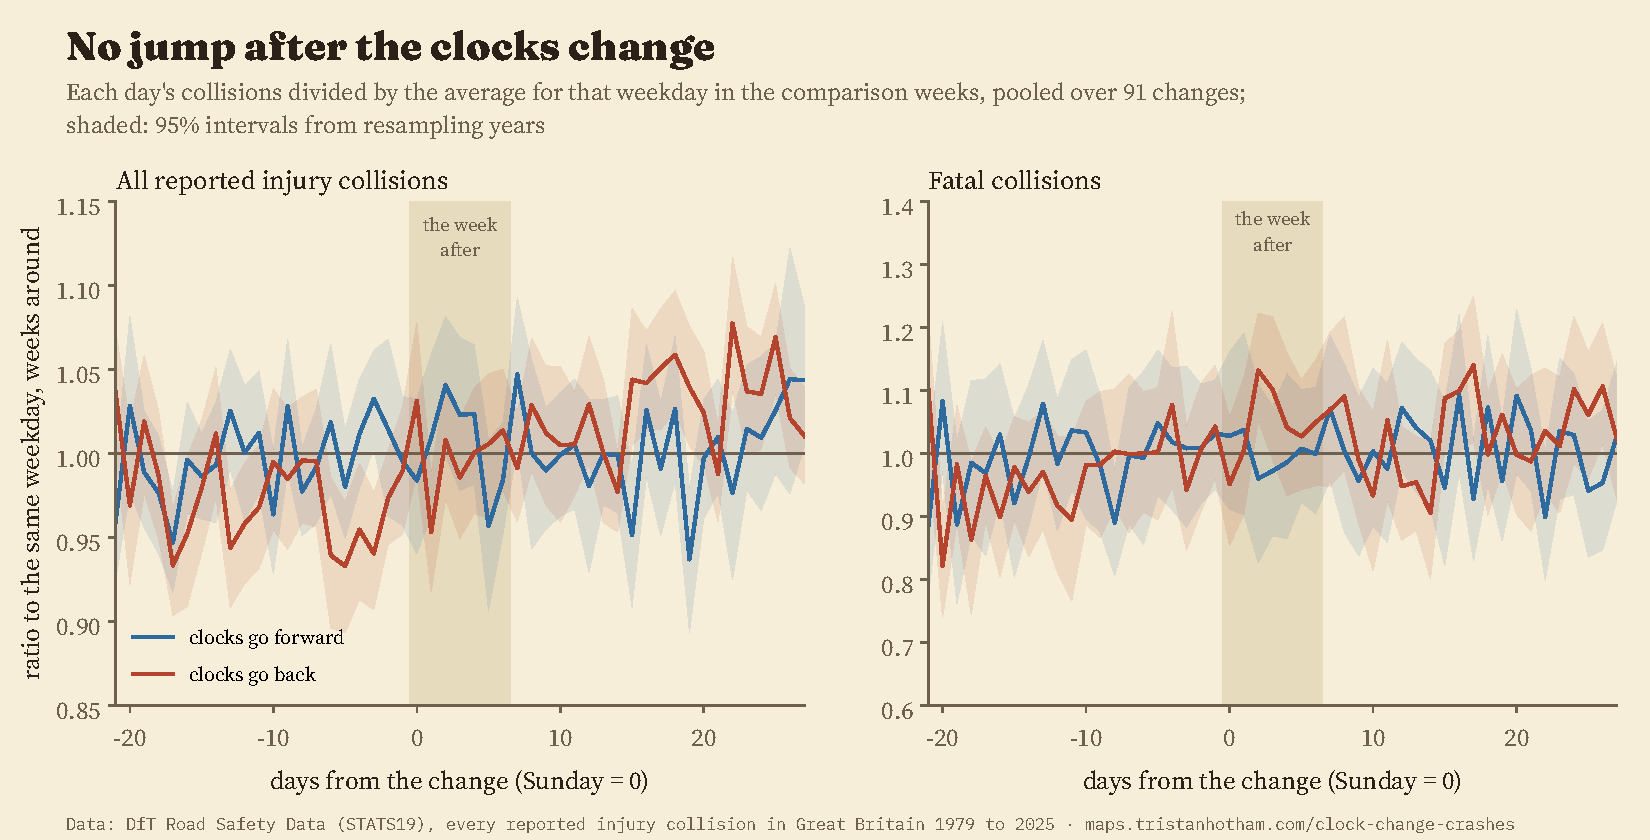
\includegraphics[width=\textwidth]{f_event.pdf}
\caption{Event study. Each day's collisions divided by the average for the same weekday in the comparison weeks, pooled over the 91 changes in the main sample, with 95\% intervals from resampling years.}\label{fig:event}
\end{figure}

\begin{figure}[tbp]\centering
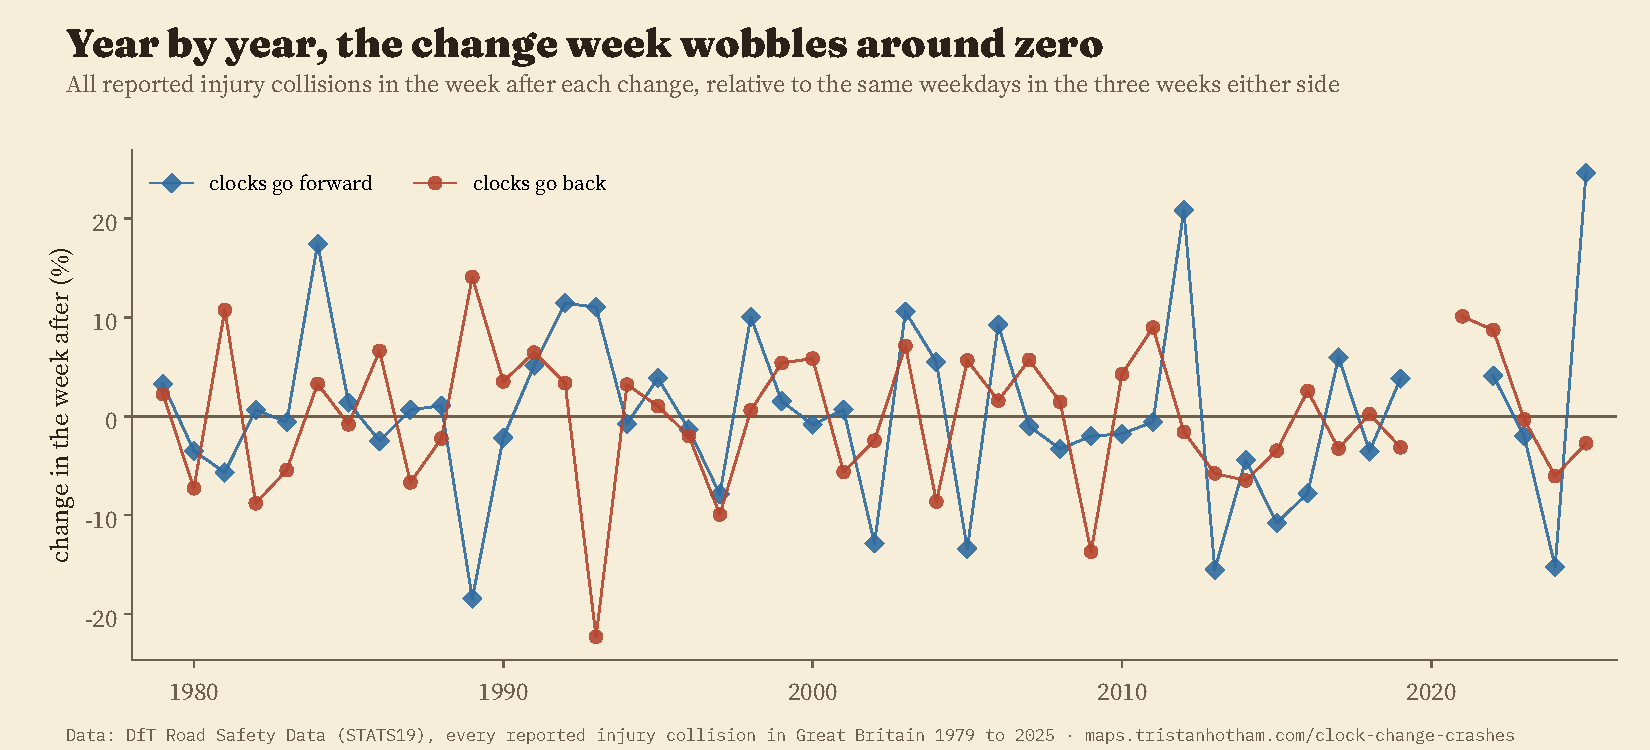
\includegraphics[width=\textwidth]{f_years.pdf}
\caption{The change-week ratio for each change, all reported injury collisions.}\label{fig:years}
\end{figure}

\subsection{The light moves}
The light effect of the change is unmistakable in the police records (Figure~\ref{fig:dark}). In the comparison weeks around the autumn change, 68\% of collisions between 17:00 and 18:59 were recorded in darkness; in the week after, 88\%. Around the spring change the evening share fell from 15\% to 4\%. The morning shares moved less, because sunrise in late March and late October is close to the start of the morning group: from 14\% to 8\% in autumn and from 1.9\% to 3.8\% in spring.

\begin{figure}[tbp]\centering
\includegraphics[width=\textwidth]{f_dark.pdf}
\caption{Share of collisions recorded in darkness by clock hour, in the comparison weeks (dashed) and the week after the change (solid).}\label{fig:dark}
\end{figure}

\subsection{Do the collisions move with the light?}
Table~\ref{tab:h2} gives the within-day estimates. After the autumn change, collisions in the evening hours rose by 3.9\% relative to the reference hours (CI 0.5 to 7.3), in the direction the darkness hypothesis predicts. For fatal collisions the point estimate is larger, 13.0\% (CI -1.4 to 29.6), but the interval includes zero. After the spring change, however, the evening hours also rose relative to midday, by 2.9\% (CI -0.1 to 6.1), although they became lighter. The morning hours fell in both seasons: by 13.3\% in autumn, when they became lighter, as predicted, and by 9.7\% in spring, when they became darker, against the prediction.

\begin{table}[tbp]\centering\footnotesize\caption{H2: collisions in each hour group in the change week relative to the reference hours (10:00 to 15:59) and to the comparison weeks. PPML with day and change-by-group fixed effects; 95\% CI clustered by year. Dark share: collisions in the group recorded in darkness, comparison weeks to change week. H3: half the autumn minus spring log difference (evening: towards darkness; morning: towards darkness), from a stacked model.}\label{tab:h2}\begin{tabular}{llrrr}\toprule Change and outcome & Hours & Rate ratio [95\% CI] & Count & Dark share\\\midrule
Clocks back (autumn), all injury & Evening 17:00 to 18:59 & 1.039 [1.005, 1.073] & 31,348 & 68\% to 88\%\\
Clocks back (autumn), all injury & Morning 06:00 to 08:59 & 0.867 [0.824, 0.913] & 23,876 & 14\% to 8\%\\
Clocks back (autumn), all injury & Other hours & 0.938 [0.914, 0.963] & 69,478 & \\
Clocks back (autumn), fatal & Evening 17:00 to 18:59 & 1.130 [0.986, 1.296] & 495 & 68\% to 88\%\\
Clocks back (autumn), fatal & Morning 06:00 to 08:59 & 1.024 [0.918, 1.142] & 327 & 14\% to 8\%\\
Clocks back (autumn), fatal & Other hours & 1.021 [0.921, 1.132] & 1,512 & \\
\midrule
Clocks forward (spring), all injury & Evening 17:00 to 18:59 & 1.029 [0.999, 1.061] & 23,842 & 15\% to 4\%\\
Clocks forward (spring), all injury & Morning 06:00 to 08:59 & 0.903 [0.825, 0.987] & 17,339 & 2\% to 4\%\\
Clocks forward (spring), all injury & Other hours & 0.988 [0.959, 1.017] & 59,084 & \\
Clocks forward (spring), fatal & Evening 17:00 to 18:59 & 0.948 [0.784, 1.147] & 266 & 15\% to 4\%\\
Clocks forward (spring), fatal & Morning 06:00 to 08:59 & 1.037 [0.851, 1.263] & 219 & 2\% to 4\%\\
Clocks forward (spring), fatal & Other hours & 0.965 [0.856, 1.088] & 1,203 & \\
\midrule
H3 darkness contrast, all injury & Evening & 1.005 [0.982, 1.028] & & \\
H3 darkness contrast, all injury & Morning & 1.020 [0.967, 1.077] & & \\
H3 darkness contrast, fatal & Evening & 1.092 [0.977, 1.219] & & \\
H3 darkness contrast, fatal & Morning & 1.006 [0.894, 1.133] & & \\
\bottomrule\end{tabular}\end{table}

Combining the seasons in the darkness contrast (H3), the evening estimate for all-injury collisions is 0.5\% (CI -1.8 to 2.8): the autumn rise and the spring rise cancel. For fatal collisions the contrast is 9.2\% (CI -2.3 to 21.9). The hour-by-hour profile (Figure~\ref{fig:hours}) shows why the groups behave as they do. In autumn the hour from 16:00 to 16:59 falls sharply and the hours from 17:00 to 18:59 rise; in spring the hour from 19:00 to 19:59, which becomes light, falls, while 17:00 to 17:59 rises. The profile also shows the mechanical effect of the change night itself, with one fewer hour between 01:00 and 01:59 in spring and one more in autumn.

\begin{figure}[tbp]\centering
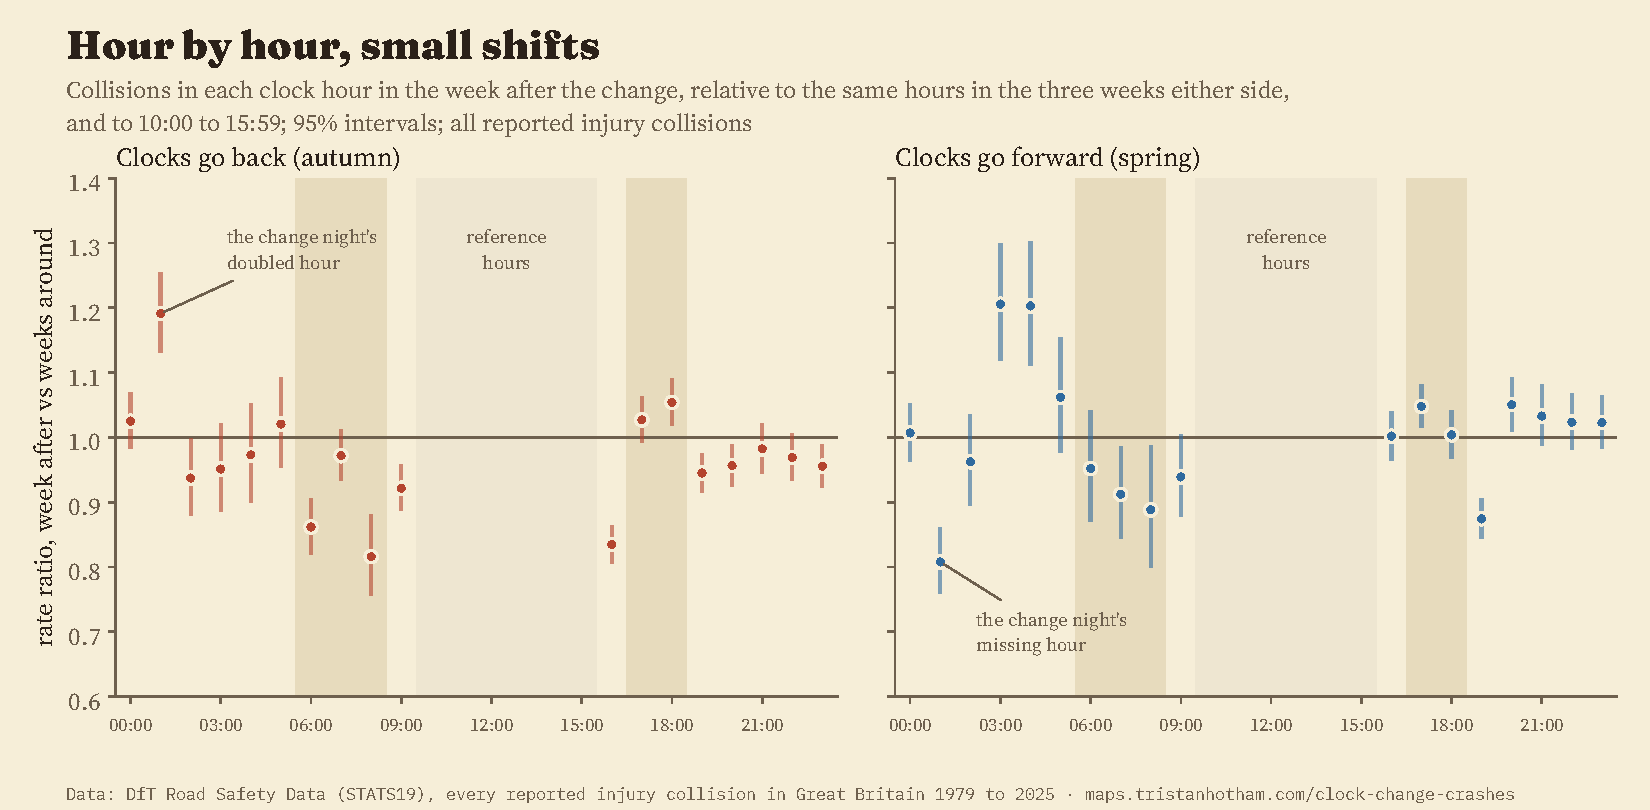
\includegraphics[width=\textwidth]{f_hours.pdf}
\caption{Hour-by-hour rate ratios: collisions in each clock hour in the week after the change, relative to the comparison weeks and to the reference hours 10:00 to 15:59. 95\% intervals, clustered by year.}\label{fig:hours}
\end{figure}

Translated into counts (H4), the autumn evening shift amounts to about 25 extra collisions in the evening hours of an average change week, against about 4,132 collisions in the whole week, and the morning shift to about 79 fewer. For fatal collisions the autumn evening estimate is about 1.2 extra fatal collisions in the evening hours per change week, against 69 in the week, with an interval that includes none.

\section{Placebo and robustness}\label{sec:robust}
\subsection{Ordinary Sundays}
Figure~\ref{fig:placebo} and Table~\ref{tab:placebo} put the real estimates beside the same estimates for 29 groups of ordinary Sundays. For all-injury collisions over the whole week, ordinary Sundays produce estimates between about $-4$\% and $+4$\%, and the real changes sit in the middle of them: 19 of 29 placebo estimates are at least as large as the spring estimate and 28 as large as the autumn one. The autumn fatal estimate is the most unusual: only 2 of 29 placebo estimates are as large. The evening estimates are not unusual: ordinary weeks move collisions between hours by several per cent as school terms, holidays and the start of the summer break change when people travel, and 7 of the 29 placebo evening estimates are at least as large as the autumn one.

\begin{figure}[tbp]\centering
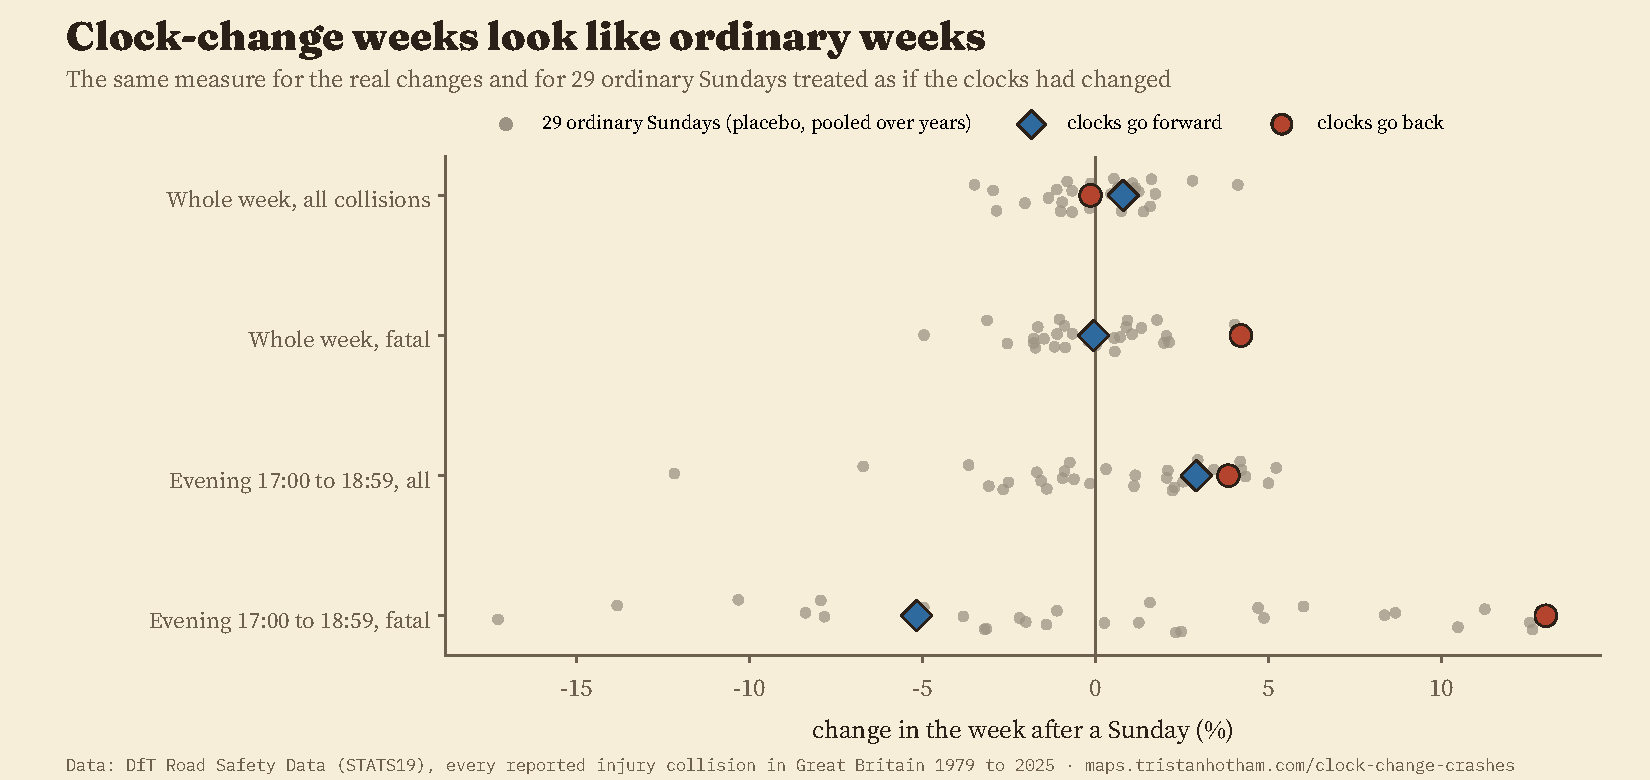
\includegraphics[width=\textwidth]{f_placebo.pdf}
\caption{The real estimates (coloured) against 29 groups of ordinary Sundays treated as if the clocks had changed (grey).}\label{fig:placebo}
\end{figure}

\begin{table}[tbp]\centering\small\caption{Real estimates against placebo Sundays pooled by ISO week. As large: placebo estimates at least as far from 1 on the log scale. CI excl.\ 1: placebo estimates whose own interval excludes 1. Largest: largest absolute placebo change (\%).}\label{tab:placebo}\begin{tabular}{lrrrr}\toprule Estimate & Real RR & As large & CI excl.\ 1 & Largest (\%)\\\midrule
Whole week, spring, all injury & 1.008 & 19 of 29 & 7 & 4.1\\
Whole week, autumn, all injury & 0.999 & 28 of 29 & 7 & 4.1\\
Whole week, spring, fatal & 1.000 & 28 of 29 & 0 & 5.2\\
Whole week, autumn, fatal & 1.042 & 2 of 29 & 0 & 5.2\\
Evening, spring, all injury & 1.029 & 11 of 29 & 14 & 13.9\\
Evening, autumn, all injury & 1.039 & 7 of 29 & 14 & 13.9\\
Evening, spring, fatal & 0.948 & 14 of 29 & 2 & 20.9\\
Evening, autumn, fatal & 1.130 & 3 of 29 & 2 & 20.9\\
Morning, spring, all injury & 0.903 & 9 of 29 & 20 & 63.7\\
Morning, autumn, all injury & 0.867 & 4 of 29 & 20 & 63.7\\
\bottomrule\end{tabular}\end{table}

\subsection{Robustness}
Table~\ref{tab:robust} and Figure~\ref{fig:robust} report the planned checks. The whole-week all-injury estimates stay between -2.4\% and 3.0\% in every check except the nation splits, and the leave-one-year-out range is 0.4\% to 1.3\% in spring and -0.6\% to 0.4\% in autumn. Three estimates have intervals that exclude zero: using only the weeks after the change as comparison gives a small autumn fall (-2.4\%, CI -4.5 to -0.2), as the seasonal trend predicts for a one-sided comparison; dropping the spring changes with Good Friday or Easter Monday in the change week gives a spring rise of 3.0\% (CI 0.3 to 5.7), which suggests that holidays in some change weeks pull the main spring estimate down and that a small spring rise cannot be ruled out; and Scotland alone (2009 to 2025) gives an autumn rise of 6.5\% (CI 1.2 to 12.2). Scotland is further north, so its autumn evenings darken earlier, but this is one of 14 nation-level estimates and was not predicted, so I do not give it weight.

The autumn fatal estimate moves between about +2\% and +9\% across checks; its interval excludes zero when the treatment window is limited to the working days (5.8\%, CI 0.8 to 11.1) and when only the weeks before are used, but not in the main specification, the casualty version or the eras. It is a suggestion, not a finding.

The hour estimates are less stable. They depend on the comparison weeks: with only the weeks before the change, the autumn evening rise is large, and with only the weeks after, it is a fall. Section~\ref{sec:step} looks at why. In the exploratory weekend-only analysis, which removes the commute and the school run, the autumn evening estimate is 4.1\% (CI -0.5 to 9.0), close to the main estimate, but the spring evening estimate is 10.0\%, again in the wrong direction for a darkness effect.

\begin{figure}[tbp]\centering
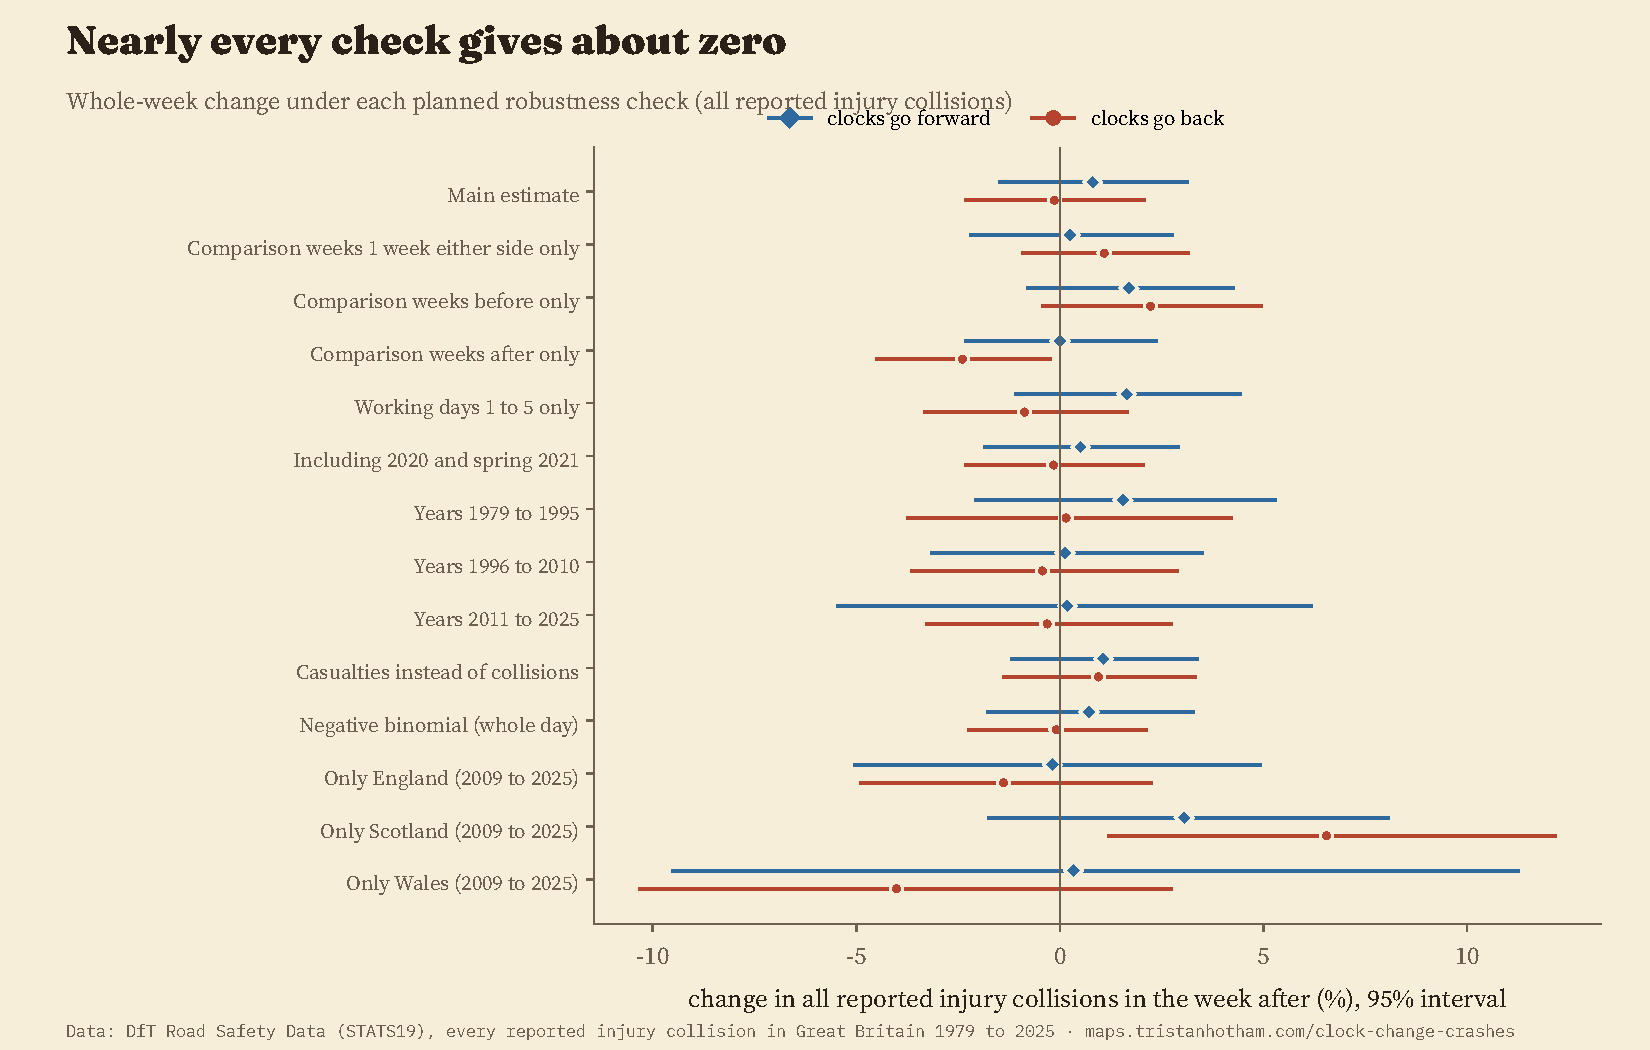
\includegraphics[width=0.95\textwidth]{f_robust.pdf}
\caption{Whole-week estimates under the planned robustness checks, all reported injury collisions, 95\% intervals.}\label{fig:robust}
\end{figure}

{\scriptsize\setlength{\tabcolsep}{3pt}\begin{longtable}{p{5.6cm}llrrr}\caption{Robustness: every planned check (and two exploratory ones), whole week (H1) and evening and morning (H2) rate ratios with 95\% CI. Nation rows use district codes, 2009 to 2025, whole-day models only.}\label{tab:robust}\\\toprule Check & Season & Outcome & Whole week & Evening & Morning\\\midrule\endhead
Comparison weeks 1 week either side only & spring & all & 1.002 [0.978, 1.027] & 1.059 [1.029, 1.090] & 0.944 [0.888, 1.004]\\
Comparison weeks 1 week either side only & spring & fatal & 0.985 [0.940, 1.032] & 0.970 [0.790, 1.191] & 1.112 [0.905, 1.366]\\
Comparison weeks 1 week either side only & autumn & all & 1.011 [0.991, 1.031] & 1.043 [1.004, 1.084] & 0.914 [0.860, 0.972]\\
Comparison weeks 1 week either side only & autumn & fatal & 1.037 [0.984, 1.093] & 1.065 [0.906, 1.252] & 0.982 [0.868, 1.110]\\
Comparison weeks before only & spring & all & 1.017 [0.992, 1.042] & 1.083 [1.050, 1.116] & 0.770 [0.711, 0.832]\\
Comparison weeks before only & spring & fatal & 1.010 [0.958, 1.066] & 0.941 [0.758, 1.168] & 0.928 [0.759, 1.136]\\
Comparison weeks before only & autumn & all & 1.022 [0.996, 1.049] & 1.195 [1.155, 1.237] & 0.921 [0.868, 0.978]\\
Comparison weeks before only & autumn & fatal & 1.068 [1.015, 1.125] & 1.535 [1.329, 1.773] & 1.048 [0.935, 1.176]\\
Comparison weeks after only & spring & all & 1.000 [0.977, 1.024] & 0.983 [0.951, 1.016] & 1.078 [0.964, 1.206]\\
Comparison weeks after only & spring & fatal & 0.993 [0.945, 1.044] & 0.953 [0.793, 1.144] & 1.164 [0.946, 1.432]\\
Comparison weeks after only & autumn & all & 0.976 [0.955, 0.998] & 0.914 [0.882, 0.948] & 0.817 [0.781, 0.855]\\
Comparison weeks after only & autumn & fatal & 1.017 [0.974, 1.062] & 0.889 [0.768, 1.030] & 0.997 [0.877, 1.133]\\
Working days 1 to 5 only & spring & all & 1.016 [0.989, 1.044] & 1.005 [0.972, 1.038] & 0.883 [0.802, 0.973]\\
Working days 1 to 5 only & spring & fatal & 0.993 [0.938, 1.052] & 0.924 [0.725, 1.177] & 1.002 [0.824, 1.219]\\
Working days 1 to 5 only & autumn & all & 0.991 [0.967, 1.016] & 1.034 [0.995, 1.075] & 0.849 [0.802, 0.899]\\
Working days 1 to 5 only & autumn & fatal & 1.058 [1.008, 1.111] & 1.123 [0.960, 1.314] & 1.051 [0.929, 1.190]\\
Including 2020 and spring 2021 & spring & all & 1.005 [0.982, 1.029] & 1.032 [1.002, 1.063] & 0.902 [0.826, 0.986]\\
Including 2020 and spring 2021 & spring & fatal & 1.002 [0.954, 1.051] & 0.963 [0.797, 1.165] & 1.028 [0.844, 1.252]\\
Including 2020 and spring 2021 & autumn & all & 0.998 [0.977, 1.020] & 1.039 [1.006, 1.074] & 0.865 [0.822, 0.911]\\
Including 2020 and spring 2021 & autumn & fatal & 1.038 [0.993, 1.085] & 1.133 [0.989, 1.297] & 1.020 [0.914, 1.138]\\
Years 1979 to 1995 & spring & all & 1.015 [0.979, 1.053] & 1.003 [0.958, 1.049] & 0.935 [0.801, 1.092]\\
Years 1979 to 1995 & spring & fatal & 0.977 [0.912, 1.046] & 0.956 [0.717, 1.276] & 1.209 [0.894, 1.634]\\
Years 1979 to 1995 & autumn & all & 1.002 [0.963, 1.042] & 1.010 [0.962, 1.060] & 0.831 [0.769, 0.897]\\
Years 1979 to 1995 & autumn & fatal & 1.029 [0.982, 1.077] & 1.153 [0.941, 1.413] & 0.980 [0.852, 1.128]\\
Years 1996 to 2010 & spring & all & 1.001 [0.969, 1.035] & 1.062 [1.005, 1.121] & 0.848 [0.728, 0.988]\\
Years 1996 to 2010 & spring & fatal & 1.027 [0.949, 1.112] & 1.040 [0.799, 1.354] & 0.941 [0.725, 1.221]\\
Years 1996 to 2010 & autumn & all & 0.996 [0.964, 1.029] & 1.058 [0.991, 1.129] & 0.923 [0.856, 0.995]\\
Years 1996 to 2010 & autumn & fatal & 1.047 [0.933, 1.174] & 1.318 [1.087, 1.599] & 1.232 [1.066, 1.423]\\
Years 2011 to 2025 & spring & all & 1.002 [0.945, 1.062] & 1.033 [0.991, 1.076] & 0.929 [0.836, 1.032]\\
Years 2011 to 2025 & spring & fatal & 1.028 [0.898, 1.176] & 0.772 [0.440, 1.352] & 0.751 [0.472, 1.194]\\
Years 2011 to 2025 & autumn & all & 0.997 [0.967, 1.027] & 1.073 [1.027, 1.121] & 0.856 [0.750, 0.978]\\
Years 2011 to 2025 & autumn & fatal & 1.085 [0.982, 1.199] & 0.793 [0.607, 1.037] & 0.849 [0.577, 1.248]\\
Spring events without Easter in the change week & spring & all & 1.030 [1.003, 1.057] & 1.084 [1.051, 1.118] & 1.097 [1.044, 1.152]\\
Spring events without Easter in the change week & spring & fatal & 0.962 [0.897, 1.032] & 0.951 [0.717, 1.260] & 1.232 [1.002, 1.514]\\
Season-specific evening (autumn 16:00 to 18:59, spring 18:00 to 19:59) & autumn & all &  & 0.968 [0.938, 0.999] & 0.867 [0.824, 0.913]\\
Season-specific evening (autumn 16:00 to 18:59, spring 18:00 to 19:59) & autumn & fatal &  & 1.019 [0.903, 1.150] & 1.024 [0.918, 1.142]\\
Season-specific evening (autumn 16:00 to 18:59, spring 18:00 to 19:59) & spring & all &  & 0.944 [0.916, 0.973] & 0.903 [0.825, 0.987]\\
Season-specific evening (autumn 16:00 to 18:59, spring 18:00 to 19:59) & spring & fatal &  & 0.832 [0.700, 0.988] & 1.037 [0.851, 1.263]\\
Exploratory: reference hours 10:00 to 13:59 & spring & all &  & 1.041 [1.003, 1.079] & 0.913 [0.830, 1.003]\\
Exploratory: reference hours 10:00 to 13:59 & spring & fatal &  & 0.950 [0.775, 1.165] & 1.039 [0.833, 1.297]\\
Exploratory: reference hours 10:00 to 13:59 & autumn & all &  & 1.012 [0.976, 1.051] & 0.845 [0.798, 0.895]\\
Exploratory: reference hours 10:00 to 13:59 & autumn & fatal &  & 1.071 [0.922, 1.244] & 0.970 [0.842, 1.118]\\
Exploratory: weekends only (no commute or school run) & spring & all &  & 1.100 [1.052, 1.150] & 0.969 [0.892, 1.052]\\
Exploratory: weekends only (no commute or school run) & spring & fatal &  & 1.007 [0.743, 1.365] & 1.109 [0.705, 1.743]\\
Exploratory: weekends only (no commute or school run) & autumn & all &  & 1.041 [0.995, 1.090] & 1.012 [0.949, 1.080]\\
Exploratory: weekends only (no commute or school run) & autumn & fatal &  & 1.145 [0.911, 1.440] & 0.884 [0.624, 1.251]\\
Casualties instead of collisions & spring & all & 1.011 [0.988, 1.034] & 1.037 [1.002, 1.073] & 0.895 [0.815, 0.983]\\
Casualties instead of collisions & spring & fatal & 0.996 [0.938, 1.058] & 0.921 [0.758, 1.120] & 0.877 [0.695, 1.106]\\
Casualties instead of collisions & autumn & all & 1.009 [0.986, 1.033] & 1.038 [1.004, 1.073] & 0.864 [0.817, 0.914]\\
Casualties instead of collisions & autumn & fatal & 1.046 [0.976, 1.121] & 1.112 [0.919, 1.345] & 0.958 [0.828, 1.109]\\
Negative binomial (whole day) & spring & all & 1.007 [0.982, 1.033] &  & \\
Negative binomial (whole day) & spring & fatal & 1.000 [0.949, 1.053] &  & \\
Negative binomial (whole day) & autumn & all & 0.999 [0.978, 1.021] &  & \\
Negative binomial (whole day) & autumn & fatal & 1.042 [0.994, 1.093] &  & \\
Nation: England & spring & all & 0.998 [0.950, 1.049] &  & \\
Nation: England & autumn & all & 0.986 [0.951, 1.022] &  & \\
Nation: Scotland & spring & all & 1.031 [0.983, 1.081] &  & \\
Nation: Scotland & autumn & all & 1.065 [1.012, 1.122] &  & \\
Nation: Wales & spring & all & 1.003 [0.905, 1.112] &  & \\
Nation: Wales & autumn & all & 0.960 [0.897, 1.027] &  & \\
Nation: Great Britain (2009 to 2025) & spring & all & 1.000 [0.953, 1.050] &  & \\
Nation: Great Britain (2009 to 2025) & autumn & all & 0.989 [0.956, 1.024] &  & \\
Leave out England (2009 to 2025) & spring & all & 1.019 [0.962, 1.080] &  & \\
Leave out England (2009 to 2025) & autumn & all & 1.023 [0.976, 1.072] &  & \\
Leave out Scotland (2009 to 2025) & spring & all & 0.998 [0.950, 1.050] &  & \\
Leave out Scotland (2009 to 2025) & autumn & all & 0.985 [0.951, 1.021] &  & \\
Leave out Wales (2009 to 2025) & spring & all & 1.000 [0.953, 1.049] &  & \\
Leave out Wales (2009 to 2025) & autumn & all & 0.990 [0.957, 1.026] &  & \\
\bottomrule\end{longtable}}


\subsection{An exploratory look at the evening step}\label{sec:step}
This subsection was not in the plan. Figure~\ref{fig:evening} shows, day by day, the evening hours' share of collisions relative to the reference hours. In both seasons the share is lower in the three weeks before the change than in the three weeks after, and it steps up on the day of the change itself. Measured against the weeks before only, the autumn evening rise is 19.5\%, larger than the same before-only estimate for any of 29 placebo weeks (largest 13.1\%). Read alone, that would be strong evidence that darkness raises evening collisions. Two things argue against reading it alone. First, the share keeps rising for three weeks after the change, by more than the step, so the change week sits below the weeks that follow; the symmetric design treats that rise as trend, and a design that compares only adjacent weeks would attribute it to the change. Second, the spring change shows a step in the same direction (before-only estimate 8.3\%), although the evening becomes lighter in spring; darkness cannot explain that. Something that moves collisions between the evening and the middle of the day around both changes, such as school holidays (the October half-term and Easter) or the change in daily routines, is at least as plausible. The planned estimate remains the main result; the step is a reason for caution in both directions.

\begin{figure}[tbp]\centering
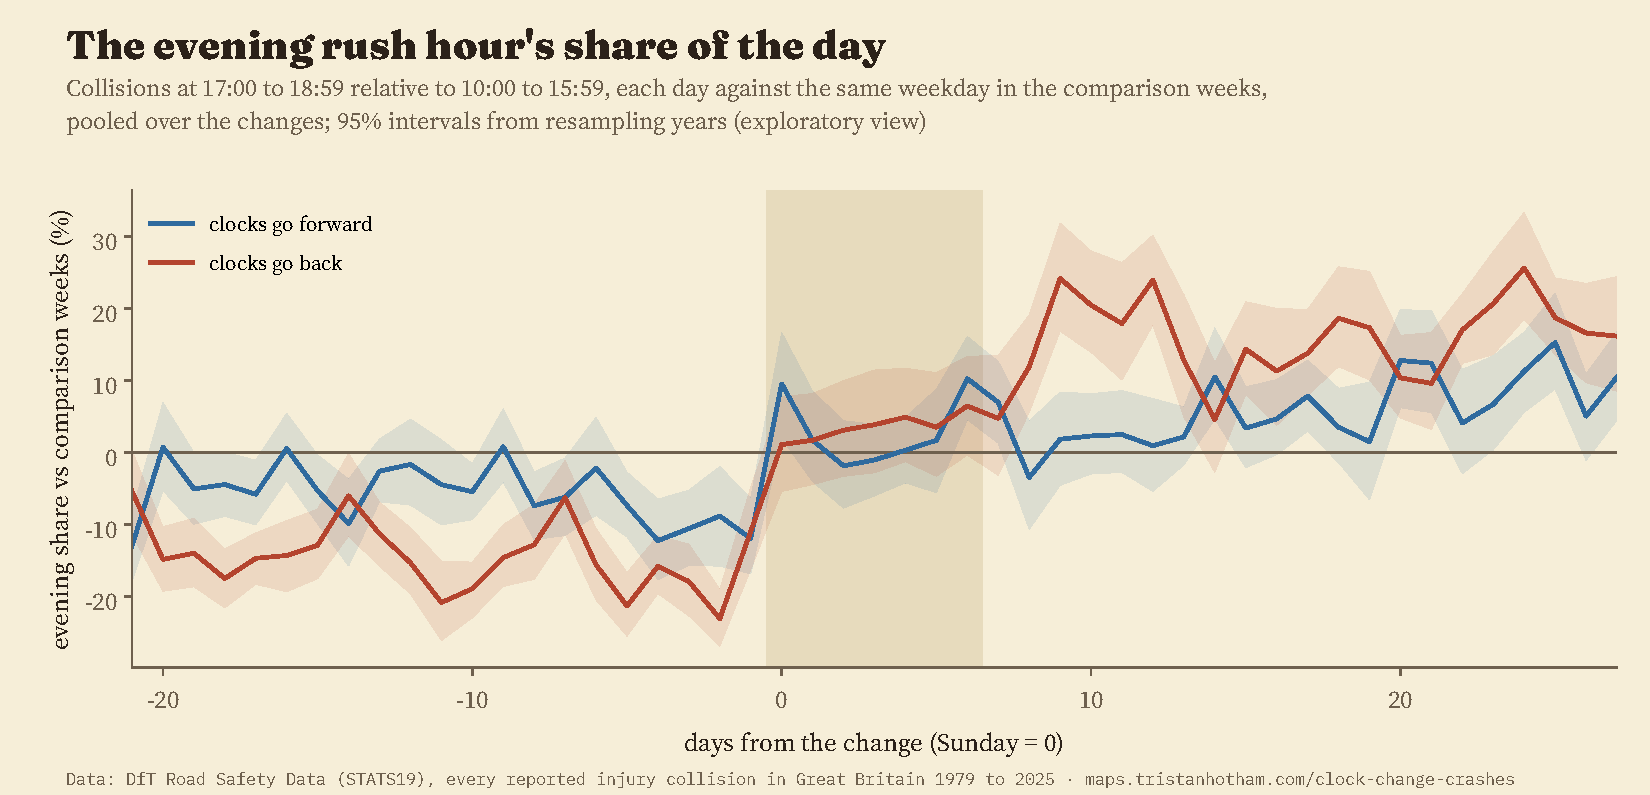
\includegraphics[width=\textwidth]{f_evening.pdf}
\caption{Exploratory: the evening hours' (17:00 to 18:59) share of each day's collisions relative to the reference hours, against the same weekday in the comparison weeks, pooled over changes, with 95\% intervals from resampling years.}\label{fig:evening}
\end{figure}

\subsection{Local authorities}
Across 349 districts and the autumn changes of 2009 to 2025, 19 district estimates have 95\% intervals excluding zero (9 above, 10 below), against about 17 expected by chance. The empirical Bayes estimates range only from 0.967 to 1.031. For spring, 15 of 350 exclude zero and the estimated between-district variance is zero. There is no evidence of local variation beyond chance (Figure~\ref{fig:map}).

\begin{figure}[tbp]\centering
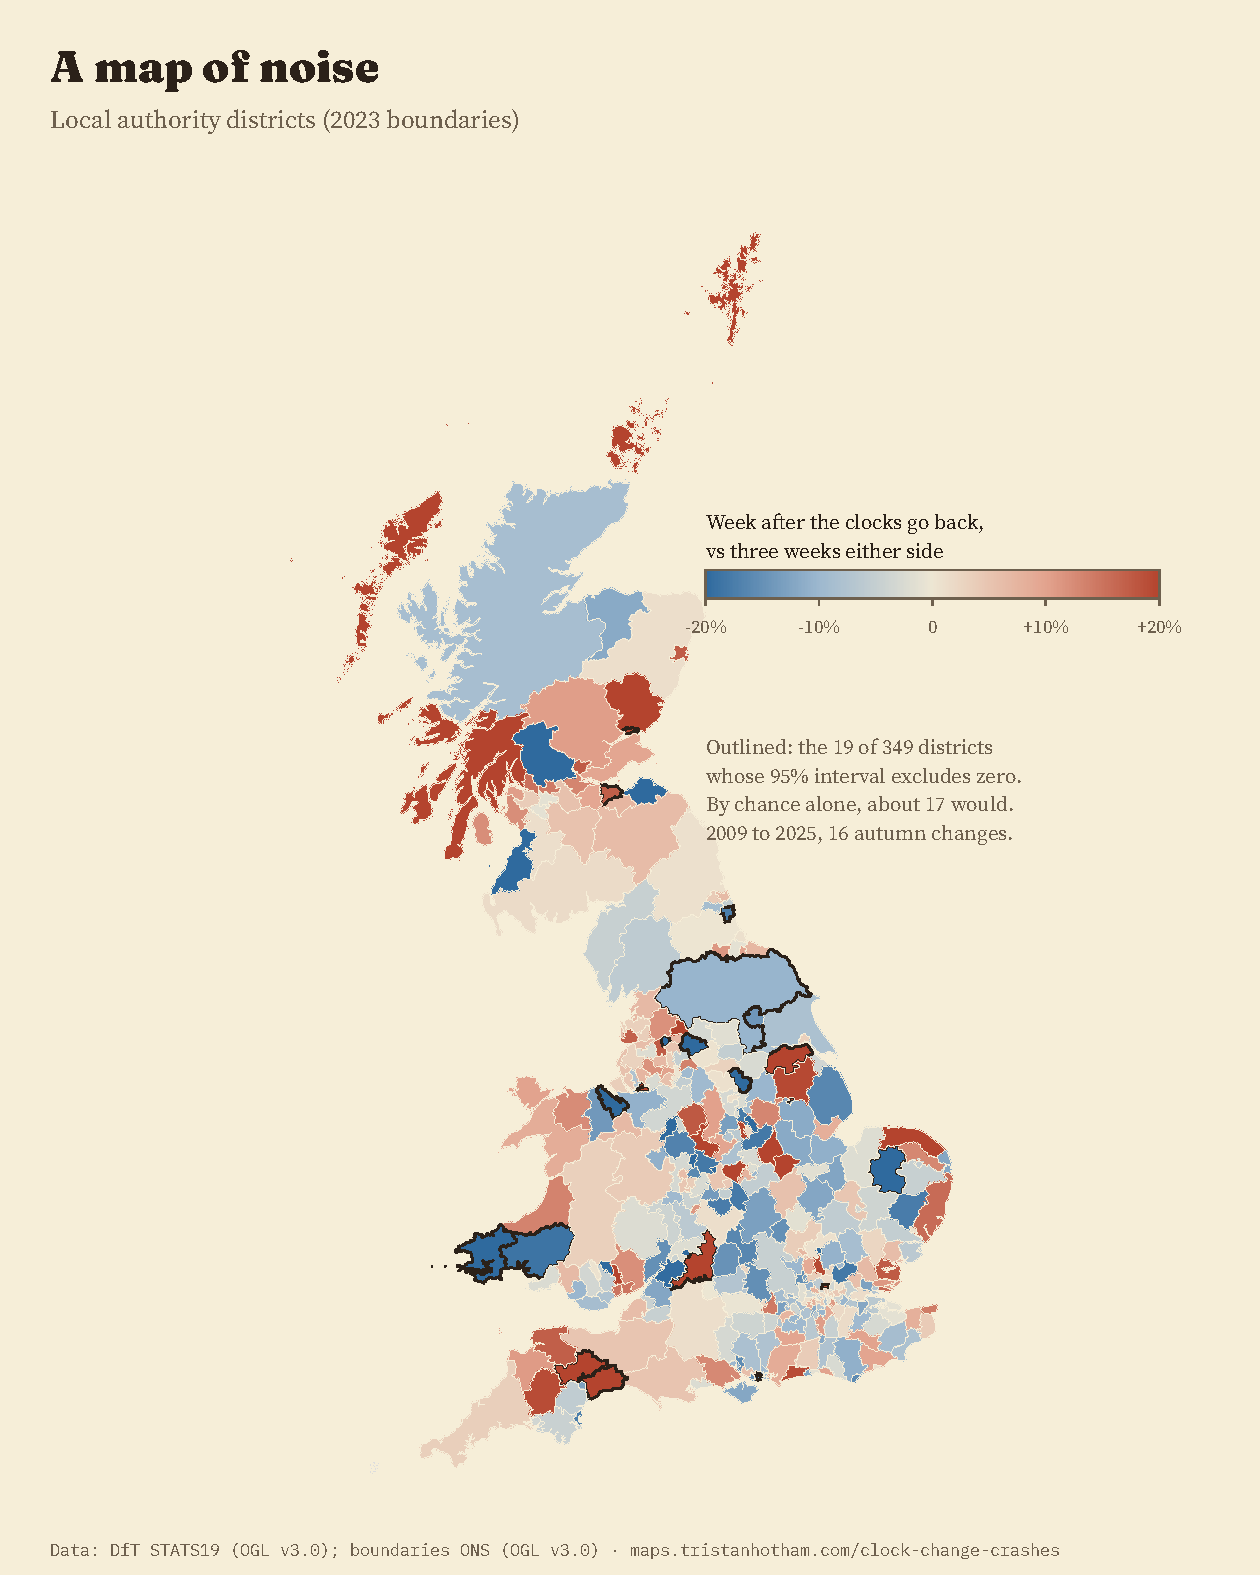
\includegraphics[width=0.62\textwidth]{f_map.pdf}
\caption{Autumn change-week rate ratio by local authority district, 2009 to 2025 (raw estimates). Outlined: intervals excluding zero.}\label{fig:map}
\end{figure}

\section{Discussion}\label{sec:disc}
\subsection{What the results say}
Over 47 years and 91 clock changes in Great Britain, the week after a clock change does not have detectably more reported injury collisions than the weeks around it. The intervals are narrow enough to rule out increases of more than about 3\% in either season. This agrees with the review by \citet{carey2017}, which found the short-run evidence inconsistent, and with the controlled design of \citet{lei2026}, which found no overall change in United States fatal crashes after the spring change. It is smaller than the six per cent rise in fatal crashes after the spring change reported by \citet{smith2016} and \citet{fritz2020}. Several differences may explain this. The United States studies use fatal crashes only, and the British fatal series here, at about 55 fatal collisions per spring change week on average, is imprecise: its interval reaches 4.9\%, so it excludes a rise of six per cent only narrowly and cannot exclude a smaller one. The British comparison window is symmetric around the change, which removes the seasonal trend that \citet{lei2026} argue inflates before-and-after estimates. And British commuting, with shorter car journeys and more public transport, may expose fewer tired drivers.

The light mechanism is real in the sense that the change moves darkness into and out of the commute. But the movement of collisions between hours is small in the planned design and inconsistent across seasons, and the exploratory step in Section~\ref{sec:step} appears in spring as well as autumn: the autumn evening rises by a few per cent, the spring evening does not fall, and ordinary weeks move collisions between hours by as much. For all-injury collisions, the combined darkness contrast for the evening is close to zero. This differs from studies that find clear light effects for pedestrians \citep{sullivan2002,uttley2017aap,woods2025}. The difference may be one of composition: most reported injury collisions involve only vehicles, for which darkness at dusk on lit urban roads matters less, and the analysis here cannot separate road users. The fatal estimates, where pedestrians are a larger share, point in the darkness direction in autumn (13\%) but are too imprecise to conclude.

\subsection{What the results do not say}
The design measures the short-run effect of the change, comparing a week with the weeks around it. It does not measure the long-run effect of where the hour of daylight sits through the winter, which is what the debate about permanent summer time is about, and which \citet{broughton1999} and \citet{bunnings2021} estimate with different designs. A null short-run effect is compatible with a real long-run effect of evening darkness, because the light is redistributed only gradually by the seasons and abruptly by the clock.

Second, the design assumes that travel stays on the clock. If people walk and cycle more in light evenings \citep{uttley2017jep}, exposure in the evening hours rises in spring and falls in autumn, which would bias the evening estimates towards zero. Without traffic counts by hour for every change, collisions per vehicle-kilometre cannot be estimated, and the estimates here are changes in counts, not in risk.

Third, the reference hours and the morning hours are touched by the school day. In England the October half-term often falls in the week after the autumn change, and Easter school holidays often overlap the spring windows. Fewer school journeys reduce collisions around 08:00 and 15:00 to 16:00, which may explain the large fall in the morning group in both seasons and the fall at 16:00 in autumn. The exploratory checks that move the reference hours or use weekends only do not change the overall conclusion, but the hour results should be read with this in mind.

Fourth, the data are police-reported collisions. Under-reporting of injury collisions to the police is substantial and varies by road user, so the results describe reported collisions only. The change in severity recording after 2012 does not affect within-year comparisons of all-injury and fatal collisions.

\subsection{Limitations of the placebo}
The placebo pools ordinary Sundays by week of the year. It shows how often normal calendar weeks produce effects of a given size, but those weeks have their own events: bank holidays, half-terms and the start of summer holidays. It is therefore a conservative benchmark for the hour estimates and an informative one for the whole-week estimates.

\section{Conclusion}\label{sec:conc}
Do the clocks kill? In Great Britain from 1979 to 2025, the weeks after the clocks change do not have more reported road injury collisions than the weeks around them. The autumn change visibly moves darkness into the evening rush hour, yet collisions in those hours rise only a few per cent relative to the middle of the day, and the spring change does not show the mirror image. The one estimate that leans towards harm, a 4\% rise in fatal collisions after the clocks go back, is uncertain and matched by 2 of 29 ordinary weeks. Whatever the case for or against changing the clocks, the short-run effect of the change itself on reported road collisions in Britain is small. The data and code are published so that the analysis can be repeated as new years are added.

\section*{Data availability statement}
Data and code: Zenodo DOI https://doi.org/10.5281/zenodo.24112857. The archive contains the event-window counts derived from STATS19 (Open Government Licence v3.0), the district panel, every estimate and the scripts that produce them. The STATS19 collision file itself is published by the Department for Transport.

\section*{AI statement}
I wrote the text, with drafting and editing assistance from Claude (Anthropic), which also helped prepare the analysis code. I reviewed and checked all text and results.

\begin{thebibliography}{99}
\bibitem[Abadie et al.(2023)]{abadie2023} Abadie, A., Athey, S., Imbens, G. W. and Wooldridge, J. M. (2023) When should you adjust standard errors for clustering? \textit{Quarterly Journal of Economics} 138(1), 1 to 35. doi:10.1093/qje/qjac038.
\bibitem[Adams et al.(2005)]{adams2005} Adams, J., White, M. and Heywood, P. (2005) Year-round daylight saving and serious or fatal road traffic injuries in children in the north-east of England. \textit{Journal of Public Health} 27(4), 316 to 317. doi:10.1093/pubmed/fdi047.
\bibitem[Barnes and Wagner(2009)]{barnes2009} Barnes, C. M. and Wagner, D. T. (2009) Changing to daylight saving time cuts into sleep and increases workplace injuries. \textit{Journal of Applied Psychology} 94(5), 1305 to 1317. doi:10.1037/a0015320.
\bibitem[Broughton and Stone(1998)]{broughton1998} Broughton, J. and Stone, M. (1998) \textit{A New Assessment of the Likely Effects on Road Accidents of Adopting SDST}. TRL Report 368. Crowthorne: Transport Research Laboratory.
\bibitem[Broughton et al.(1999)]{broughton1999} Broughton, J., Hazelton, M. and Stone, M. (1999) Influence of light level on the incidence of road casualties and the predicted effect of changing `summertime'. \textit{Journal of the Royal Statistical Society: Series A} 162(2), 137 to 175. doi:10.1111/1467-985X.00128.
\bibitem[B\"unnings and Schiele(2021)]{bunnings2021} B\"unnings, C. and Schiele, V. (2021) Spring forward, don't fall back: the effect of daylight saving time on road safety. \textit{Review of Economics and Statistics} 103(1), 165 to 176. doi:10.1162/rest\_a\_00873.
\bibitem[Cameron and Miller(2015)]{cameron2015} Cameron, A. C. and Miller, D. L. (2015) A practitioner's guide to cluster-robust inference. \textit{Journal of Human Resources} 50(2), 317 to 372.
\bibitem[Carey and Sarma(2017)]{carey2017} Carey, R. N. and Sarma, K. M. (2017) Impact of daylight saving time on road traffic collision risk: a systematic review. \textit{BMJ Open} 7(6), e014319. doi:10.1136/bmjopen-2016-014319.
\bibitem[Coate and Markowitz(2004)]{coate2004} Coate, D. and Markowitz, S. (2004) The effects of daylight and daylight saving time on US pedestrian fatalities and motor vehicle occupant fatalities. \textit{Accident Analysis and Prevention} 36(3), 351 to 357. doi:10.1016/S0001-4575(03)00015-0.
\bibitem[Coren(1996)]{coren1996} Coren, S. (1996) Daylight savings time and traffic accidents. \textit{New England Journal of Medicine} 334(14), 924. doi:10.1056/NEJM199604043341416.
\bibitem[Correia et al.(2020)]{correia2020} Correia, S., Guimar\~aes, P. and Zylkin, T. (2020) Fast Poisson estimation with high-dimensional fixed effects. \textit{Stata Journal} 20(1), 95 to 115. doi:10.1177/1536867X20909691.
\bibitem[Department for Transport(2026a)]{dft2026} Department for Transport (2026a) Road safety data: dft-road-casualty-statistics-collision-1979-latest-published-year.csv. data.gov.uk, retrieved 2026. Open Government Licence v3.0.
\bibitem[Department for Transport(2026b)]{dftseverity2026} Department for Transport (2026b) Guide to severity adjustments for reported road casualties Great Britain. GOV.UK, first published 2021, updated 2026.
\bibitem[DerSimonian and Laird(1986)]{dersimonian1986} DerSimonian, R. and Laird, N. (1986) Meta-analysis in clinical trials. \textit{Controlled Clinical Trials} 7(3), 177 to 188. doi:10.1016/0197-2456(86)90046-2.
\bibitem[European Parliament and Council(2001)]{eu2001} European Parliament and Council of the European Union (2001) Directive 2000/84/EC of 19 January 2001 on summer-time arrangements. \textit{Official Journal of the European Communities} L 31.
\bibitem[Ferguson et al.(1995)]{ferguson1995} Ferguson, S. A., Preusser, D. F., Lund, A. K., Zador, P. L. and Ulmer, R. G. (1995) Daylight saving time and motor vehicle crashes: the reduction in pedestrian and vehicle occupant fatalities. \textit{American Journal of Public Health} 85(1), 92 to 95. doi:10.2105/AJPH.85.1.92.
\bibitem[Fritz et al.(2020)]{fritz2020} Fritz, J., VoPham, T., Wright, K. P. and Vetter, C. (2020) A chronobiological evaluation of the acute effects of daylight saving time on traffic accident risk. \textit{Current Biology} 30(4), 729 to 735. doi:10.1016/j.cub.2019.12.045.
\bibitem[Hansard(1970)]{hansard1970} Hansard (1970) British Standard Time. Written answer, House of Commons, 27 November 1970, vol. 807, col. 234W.
\bibitem[Harrison(2013)]{harrison2013} Harrison, Y. (2013) The impact of daylight saving time on sleep and related behaviours. \textit{Sleep Medicine Reviews} 17(4), 285 to 292. doi:10.1016/j.smrv.2012.10.001.
\bibitem[Hicks et al.(1983)]{hicks1983} Hicks, R. A., Lindseth, K. and Hawkins, J. (1983) Daylight saving-time changes increase traffic accidents. \textit{Perceptual and Motor Skills} 56(1), 64 to 66. doi:10.2466/pms.1983.56.1.64.
\bibitem[Home Office(1970)]{homeoffice1970} Home Office (1970) \textit{Review of British Standard Time}. Cmnd 4512. London: HMSO.
\bibitem[Huang and Levinson(2010)]{huang2010} Huang, A. and Levinson, D. (2010) The effects of daylight saving time on vehicle crashes in Minnesota. \textit{Journal of Safety Research} 41(6), 513 to 520. doi:10.1016/j.jsr.2010.10.006.
\bibitem[IANA(2026)]{iana2026} IANA (2026) Time Zone Database (tz), zone Europe/London, as distributed with Python zoneinfo. Internet Assigned Numbers Authority, retrieved 2026.
\bibitem[Janszky and Ljung(2008)]{janszky2008} Janszky, I. and Ljung, R. (2008) Shifts to and from daylight saving time and incidence of myocardial infarction. \textit{New England Journal of Medicine} 359(18), 1966 to 1968. doi:10.1056/NEJMc0807104.
\bibitem[Johansson et al.(2009)]{johansson2009} Johansson, \"O., Wanvik, P. O. and Elvik, R. (2009) A new method for assessing the risk of accident associated with darkness. \textit{Accident Analysis and Prevention} 41(4), 809 to 815.
\bibitem[Kantermann et al.(2007)]{kantermann2007} Kantermann, T., Juda, M., Merrow, M. and Roenneberg, T. (2007) The human circadian clock's seasonal adjustment is disrupted by daylight saving time. \textit{Current Biology} 17(22), 1996 to 2000. doi:10.1016/j.cub.2007.10.025.
\bibitem[Lahti et al.(2010)]{lahti2010} Lahti, T., Nysten, E., Haukka, J., Sulander, P. and Partonen, T. (2010) Daylight saving time transitions and road traffic accidents. \textit{Journal of Environmental and Public Health} 2010, 657167. doi:10.1155/2010/657167.
\bibitem[Laliotis et al.(2023)]{laliotis2023} Laliotis, I., Moscelli, G. and Monastiriotis, V. (2023) Summertime and the drivin' is easy? Daylight saving time and vehicle accidents. \textit{Health Economics} 32(10), 2192 to 2215. doi:10.1002/hec.4715.
\bibitem[Lambe and Cummings(2000)]{lambe2000} Lambe, M. and Cummings, P. (2000) The shift to and from daylight savings time and motor vehicle crashes. \textit{Accident Analysis and Prevention} 32(4), 609 to 611. doi:10.1016/S0001-4575(99)00088-3.
\bibitem[Lei et al.(2026)]{lei2026} Lei, D., Du, Y., Peng, S. and Zhang, M. (2026) Does daylight saving time increase traffic crashes? Seasonal confounding and a morning fatality effect. \textit{Accident Analysis and Prevention} 237, 108719. doi:10.1016/j.aap.2026.108719.
\bibitem[Meyerhoff(1978)]{meyerhoff1978} Meyerhoff, N. J. (1978) The influence of daylight saving time on motor vehicle fatal traffic accidents. \textit{Accident Analysis and Prevention} 10(3), 207 to 221. doi:10.1016/0001-4575(78)90012-X.
\bibitem[mySociety(2026)]{mysociety2026} mySociety (2026) UK local authority names and codes (uk\_local\_authorities.csv). GitHub, github.com/mysociety/uk\_local\_authority\_names\_and\_codes, retrieved 2026. CC BY 4.0.
\bibitem[Plainis et al.(2006)]{plainis2006} Plainis, S., Murray, I. J. and Pallikaris, I. G. (2006) Road traffic casualties: understanding the night-time death toll. \textit{Injury Prevention} 12(2), 125 to 128. doi:10.1136/ip.2005.011056.
\bibitem[Robb and Barnes(2018)]{robb2018} Robb, D. and Barnes, T. (2018) Accident rates and the impact of daylight saving time transitions. \textit{Accident Analysis and Prevention} 111, 193 to 201. doi:10.1016/j.aap.2017.11.029.
\bibitem[Santos Silva and Tenreyro(2006)]{santos2006} Santos Silva, J. M. C. and Tenreyro, S. (2006) The log of gravity. \textit{Review of Economics and Statistics} 88(4), 641 to 658. doi:10.1162/rest.88.4.641.
\bibitem[Smith(2016)]{smith2016} Smith, A. C. (2016) Spring forward at your own risk: daylight saving time and fatal vehicle crashes. \textit{American Economic Journal: Applied Economics} 8(2), 65 to 91. doi:10.1257/app.20140100.
\bibitem[Sood and Ghosh(2007)]{sood2007} Sood, N. and Ghosh, A. (2007) The short and long run effects of daylight saving time on fatal automobile crashes. \textit{B.E. Journal of Economic Analysis and Policy} 7(1). doi:10.2202/1935-1682.1618.
\bibitem[Stevens and Lord(2006)]{stevens2006} Stevens, C. R. and Lord, D. (2006) Evaluating safety effects of daylight savings time on fatal and nonfatal injury crashes in Texas. \textit{Transportation Research Record} 1953, 147 to 155. doi:10.3141/1953-17.
\bibitem[Sullivan and Flannagan(2002)]{sullivan2002} Sullivan, J. M. and Flannagan, M. J. (2002) The role of ambient light level in fatal crashes: inferences from daylight saving time transitions. \textit{Accident Analysis and Prevention} 34(4), 487 to 498. doi:10.1016/S0001-4575(01)00046-X.
\bibitem[Sullivan and Flannagan(2007)]{sullivan2007} Sullivan, J. M. and Flannagan, M. J. (2007) Determining the potential safety benefit of improved lighting in three pedestrian crash scenarios. \textit{Accident Analysis and Prevention} 39(3), 638 to 647. doi:10.1016/j.aap.2006.10.010.
\bibitem[Summer Time Act(1972)]{summertimeact1972} Summer Time Act 1972 (c. 6). legislation.gov.uk/ukpga/1972/6.
\bibitem[Uttley and Fotios(2017a)]{uttley2017aap} Uttley, J. and Fotios, S. (2017a) The effect of ambient light condition on road traffic collisions involving pedestrians on pedestrian crossings. \textit{Accident Analysis and Prevention} 108, 189 to 200. doi:10.1016/j.aap.2017.09.005.
\bibitem[Uttley and Fotios(2017b)]{uttley2017jep} Uttley, J. and Fotios, S. (2017b) Using the daylight savings clock change to show ambient light conditions significantly influence active travel. \textit{Journal of Environmental Psychology} 53, 1 to 10. doi:10.1016/j.jenvp.2017.06.003.
\bibitem[Varughese and Allen(2001)]{varughese2001} Varughese, J. and Allen, R. P. (2001) Fatal accidents following changes in daylight savings time: the American experience. \textit{Sleep Medicine} 2(1), 31 to 36. doi:10.1016/S1389-9457(00)00032-0.
\bibitem[Whittaker(1996)]{whittaker1996} Whittaker, J. D. (1996) An investigation into the effects of British Summer Time on road traffic accident casualties in Cheshire. \textit{Journal of Accident and Emergency Medicine} 13(3), 189 to 192. doi:10.1136/emj.13.3.189.
\bibitem[Woods et al.(2025)]{woods2025} Woods, A. N., Weast, R. A. and Monfort, S. S. (2025) Daylight saving time and fatal crashes: the impact of changing light conditions. \textit{Journal of Safety Research} 93, 200 to 205. doi:10.1016/j.jsr.2025.02.010.
\end{thebibliography}

\appendix
\section{Appendix: further tables and data construction}
\begin{table}[htbp]\centering\small\caption{Leave one year out: range of the planned estimates when each year's change is dropped in turn.}\label{tab:appx}\begin{tabular}{llrrr}\toprule Season & Outcome & Whole week & Evening & Morning\\\midrule
spring & all & 1.004 to 1.013 & 1.023 to 1.034 & 0.891 to 0.915\\
spring & fatal & 0.990 to 1.009 & 0.895 to 0.983 & 0.989 to 1.062\\
autumn & all & 0.994 to 1.004 & 1.031 to 1.045 & 0.861 to 0.874\\
autumn & fatal & 1.033 to 1.052 & 1.110 to 1.164 & 1.006 to 1.039\\
\bottomrule\end{tabular}\end{table}

Table~\ref{tab:appx} gives the leave-one-year-out ranges and the secondary estimates. \textbf{Data construction.} The STATS19 collision file was reduced to an array of counts by day (17,532 days from 1 January 1979), clock hour (0 to 23; no collision lacks a time), severity (fatal, serious, slight) and light condition (daylight; any darkness category; unknown), and to a second array summing casualties, and a third counting collisions by local authority district code. Eight malformed rows of the source file were dropped. Bank holidays are those of England and Wales, computed from the Easter date and the statutory rules with the special holidays of 1981, 1999, 2002, 2011, 2012, 2022 and 2023. \textbf{Software.} Python 3 with pandas, numpy, pyfixest (Poisson pseudo-maximum likelihood with high-dimensional fixed effects), statsmodels (negative binomial), matplotlib and xelatex.

\end{document}
